\documentclass[main]{subfiles}

\begin{document}


\chapter{Diseño del controlador}
\label{chap:control}

Diversas técnicas de control nos permiten alcanzar el objetivo trazado de lograr que el cuadric\'optero siga alguna de las trayectorias espec\'ificadas en el cap\'itulo \ref{chap:linealizacion}. En lo que respecta al control lineal y de acuerdo a la bibliograf\'ia estudiada, dos técnicas son principalmente utilizadas, control PID\footnote{Proporcional, integral y derivativo} y LQR\footnote{Linear quadratic regulator}. Ambas t\'ecnicas presentan ventajas y desventajas. En el trabajo realizado en \ref{bib:quadrotor-bible} se propone el control de un cuadric\'optero utilizando un controlador PID. La gran mayoría de controladores en aplicaciones industriales son de este tipo, la principal ventaja que presentan es que se trata de un diseño que tiene una estructura simple y es adecuado para la gran mayoría de procesadores ya que el costo computacional del mismo es prácticamente nulo. En dicho t\'ecnica de control la señal de entrada a la planta es una funci\'on del error entre el estado deseado y el estado estimado.
\begin{equation}
u(t) = K_pe(t)+K_I\int_0^t e(\tau) d\tau +K_d\frac{de(t)}{dt}
\end{equation}

donde $e(t) = X_d-\hat{X}$.

Es fundamental en esta t\'ecnica de control la determinaci\'on de las constantes. En \ref{bib:quadrotor-bible} se limitan las trayectorias a trayectorias de hovering. En ese supuesto, se realizan algunas aproximaciones que permiten reducir el sistema f\'isico a las siguientes ecuaciones
\begin{equation}
\left(
\begin{array}{c}
\ddot{z}\\
\ddot{\psi}\\
\ddot{\varphi} \\
\ddot{\theta}
\end{array}\right)
=\left(\begin{array}{c}
g+(\cos\varphi\cos\psi)\frac{U_1}{M}\\
 \frac{U_2}{I_{xx}} \\
 \frac{U_3}{I_{yy}} \\
 \frac{U_4}{I_{zz}} \\
\end{array}\right)
\end{equation}

Donde $U_1, U_2, U_3$ y $U_4$ son combinaciones lineales de los cuadrados de las velocidades angulares de cada motor. En este caso se puede tratar cada variable por separado, ya que cada variable es afectada por una sola entrada, siendo relativamente sencillo determinar las constantes $K_p, K_I$ y $K_d$ en funci\'on de donde se desea ubicar los polos del sistema realimentado. Con esta estrategia se pierde la posibilidad de controlar las otras 8 variables de estado, limit\'andose entonces a un cuadric\'optero que puede realizar exclusivamente movimientos en la direcci\'on vertical y giros en torno a su eje vertical.\\

Si se intenta controlar el sistema de inter\'es en este trabajo utilizando esta t\'ecnica, nos enfrentar\'iamos al problema de determinar al menos una matriz de realimentaci\'on (si trabajamos solamente con un controlador proporcional). Dicha matriz, debe ser de $12\times4$, es decir que se deben determinar los 48 elementos de la matriz de forma de lograr que la respuesta del sistema sea la deseada. Esta tarea no resulta sencilla, ya que es extremadamente dificultoso comprender exactamente la influencia de cada par\'ametro de la matriz de realimentaci\'on en la ubicaci\'on de los polos en el sistema realimentado incluso para asegurar algo elemental y necesario como la estabilidad del sistema.\\

Por dicho motivo se opto por explorar el camino propuesto por otros trabajos como \ref{bib:lqr-discreto}, donde la t\'ecnica elegida para realizar el control del cuadric\'optero es LQR.


\section{Conceptos generales sobre LQR}

Consideremos el sistema realimentado de la figura \ref{fig:bloque}, con $X(t)\in \mathcal{M}_{n\times1}$el vector de estados del sistema y $u(t)\in \mathcal{M}_{m\times1}$ las entradas. $r$ es el setpoint del cual, multiplicando por dos matrices adecuadas pueden obtenerse los valores deseados de entrada $u^*$ y de las variables de estado $X^*$. El objetivo que nos planteamos es el de obtener una matriz de realimentaci\'on K para el sistema utilizando la t\'ecnica de LQR. 

     
\begin{figure}
	\centering
	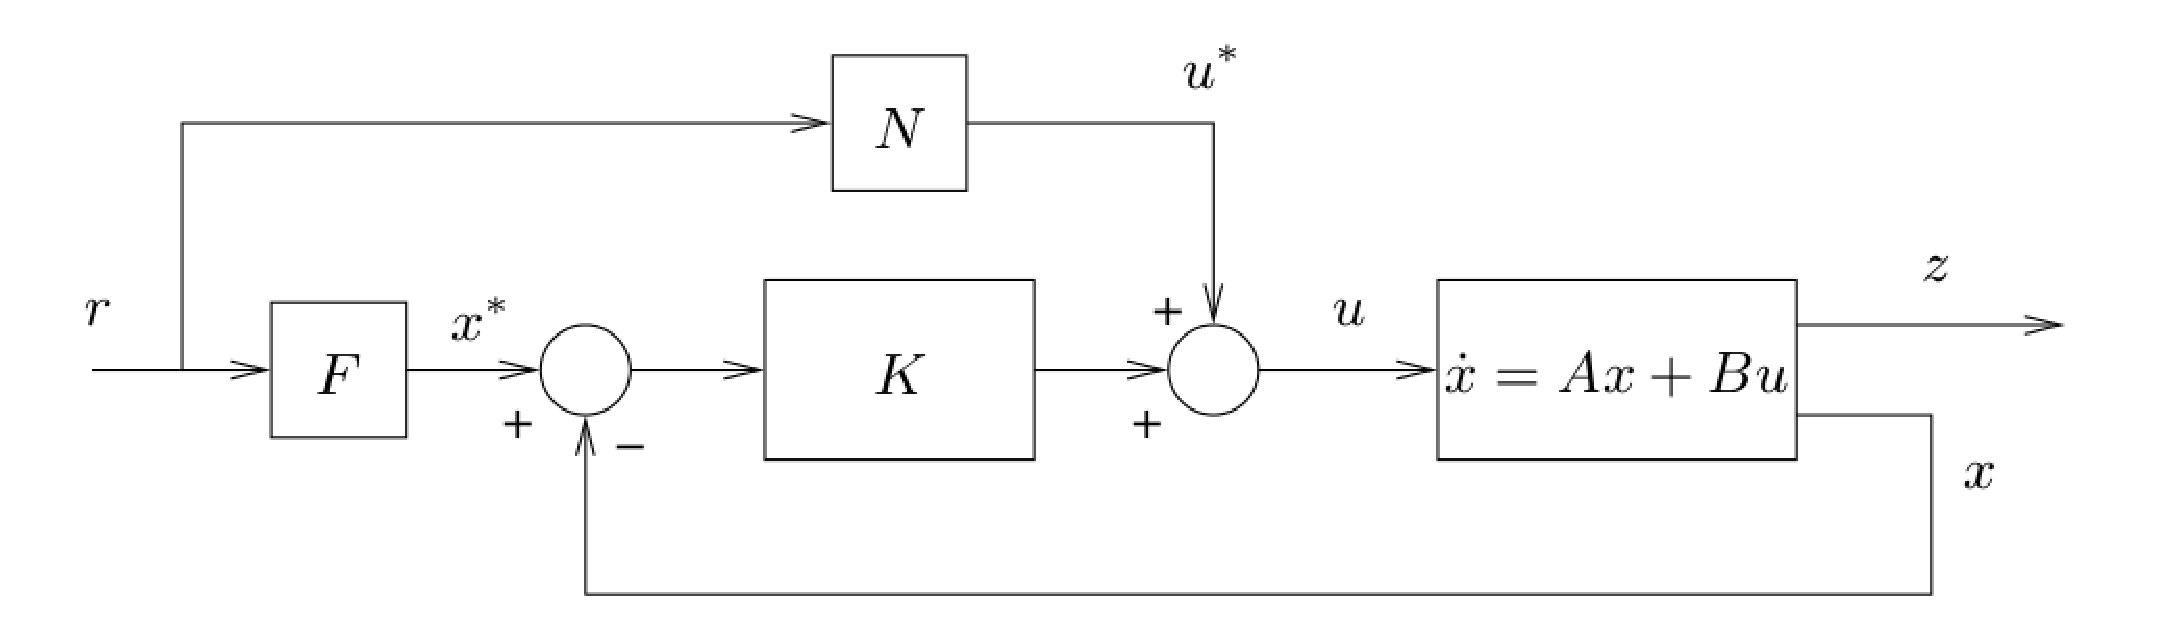
\includegraphics[width=0.7\textwidth]{./pics_control/bloque.pdf}
	\caption{Sistema realimentado}
	\label{fig:bloque}
\end{figure}
 
El problema de encontrar un regulador \'optimo puede plantearse de la siguiente forma; se trata de encontrar la matriz de transferencia $C(s)$ que minimice la siguiente funci\'on de costo:

\begin{equation}
\label{eq:lqr}
J_{LQR} = \int_{0}^{\infty}  X'(t)Q X(t)+u'(t)Ru(t)dt
\end{equation}

Donde $Q$ y $R$ son matrices sim\'etricas definidas positivas de dimensiones $n\times n$ y $m\times m$ respectivamente. Cabe aclarar que esta es la formulaci\'on para el problema LQR continuo y de horizonte infinito. 


El primer t\'ermino de la integral corresponde a la energ\'ia de los estados controlados y el segundo a la energ\'ia de la señal de control. En funci\'on de como se escogen las matrices $Q$ y $R$, se obtienen resultados distintos. Por ejemplo si la norma de $Q$ es pequeña la forma m\'as efectiva de reducir $J_{LQR}$ es utilizar señales de control de norma pequeña a expensas de tener grandes variaciones en los estados controlados. Si bien existen diversos m\'etodos para determinar las matrices $Q$ y $R$, gran parte del trabajo es iterativo y se realiza a ensayo y error\\  

En la versi\'on de realimentaci\'on de estados del problema LQR se asume que se disponen de medidas de todas las variables del vector de estados. En este caso, el controlador \'optimo LQR es una matriz de ganancia K tal que:
\begin{equation}
u(t)-u^*(t) = -K(X(t)-X^*(t))
\end{equation}

Donde $K\in\mathcal{M}_{m\times n}$. Para el caso bajo an\'alisis se tiene que: 

\begin{equation}
K = R^{-1}B^TP
\end{equation}

Donde P es la soluci\'on a la ecuaci\'on algebraica de Riccati.

La propiedad escencial del controlador LQR es que la respuesta del sistema en lazo cerrado es asint\'oticamente estable, es decir que la parte real de los valores propios de la matriz $A-BK$ es negativa, mientras se cumplan las siguientes condiciones:

\begin{itemize}
\item El sistema es controlable
\item El sistema es observable
\end{itemize}.

\section{Consideraciones particulares respecto del sistema a controlar}

Como se explico en cap\'itulos anteriores, se tienen una nueva estimaci\'on del vector de estados cada $10 ms$ esto nos permite realizar acciones de control con esta misma tasa de muestreo. De acuerdo a las constantes de tiempo que involucra el sistema f\'isico se puede afirmar que es un tiempo de acci\'on adecuado para trabajar. A modo de ejemplo consideremos la variable $\omega_{q_z}$. De acuerdo a las velocidades angulares de los motores que se utilizar\'an ($109 rads^{-1} < w_i < 387 rads^{-1})$ y suponiendo que nos encontramos trabajando a la velocidad angular de equilibrio ($334.28 rads^{-1}$ La aceleraci\'on angular m\'axima que puede darse es de $20.2 rad s^{-2}$. En el tiempo de muestreo implica un cambio en la velocidad angular de $11.5 ^{\circ} s^{-1}$ y un cambio en el \'angulo de Yaw de $0.058^{\circ}$. Estas pequeñas variaciones nos indican que el tiempo de acci\'on escogido es adecuado. Esto ser\'a confirmado posterioremente con las simulaciones realizadas. \\

Al tener un tiempo de respuesta r\'apido (en relaci\'on a las constantes del sistema) se podr\'ia resolver el problema utilizando la t\'ecnica de control LQR pensando en un sistema continuo, por m\'as que nuestro sistema sea un sistema discreto. Sin embargo los m\'etodos m\'as sencillos para determinar la matriz de realimentaci\'on se encontraron utilizando algor\'itmos basados en LQR discreto. Esto fue determinante a la hora de escoger la t\'ecnica de control.\\

Por otra parte, el problema LQR tiene una versi\'on de horizonte finito y una versi\'on de horizonte finito. A lo largo del tiempo iremos cambiando el setpoint del sistema cada ciertos intervalos de tiempo. Por dicho motivo, el horizonte de nuestro sistema es en sentido estricto de horizonte finito. Sin embargo, las constantes de tiempo involucradas nos permiten asumir que se trata de un sistema de horizonte infinito, lo cual nos permite simplificar las ecuaciones con las que se trabaja.\\

\section{Discretizaci\'on del sistema}

Como se explic\'o en el cap\'itulo \ref{chap:linealizacion} se trabjar\'a con tres tipos de trayectoria: hovering, vuelos en linea recta y c\'irculos. En cada uno de estos casos tenemos un sistema lineal de la forma 
\begin{equation}
\dot{X} = A X + Bu
\end{equation}
 
La forma que toma el sistema continuo al ser convertido a tiempo discreto es: 

\begin{equation}
X_{k+1} = \Phi X_k + \Gamma u_k
\end{equation}
Donde:
\begin{equation}
\Phi = e^{AT_s} \quad \Gamma = \int_0^{T_s} e^{A s} ds B
\end{equation}
Estas relaciones surgen de discretizar el sistema considerando muestreadores de \'orden cero. Por m\'as detalles de este proceso puede consultarse \ref{bib:hakas}.\\

El problema de encontrar un regulador \'optimo tambi\'en puede ser planteado en un sisetma discreto si reescribimos la ecuaci\'on \ref{eq:lqr}. 
\begin{equation}
\label{eq:dlqr}
J_{dlqr} = \sum_0^\infty x_k^T Q x_k + u_k^T R u_k
\end{equation}

En el trabajo realizado en \ref{bib:lqr-discreto} se propone un algoritmo iterativo para obtener la matriz de realimentaci\'on que minimiza $J_{dlqr}$. Debido a las pequeñas diferencias encontradas entre este algor\'itmo y la funci\'on \emph{lqrd} de \emph{MatLab}  se opt\'o por reproducir exactamente dicho algor\'itmo.

\section{Controlabilidad y observabilidad}

Los conceptos de controlabilidad y observabilidad son fundamentales para asegurar la estabilidad del sistema en lazo cerrado controlado con la t\'ecnica de LQR.\\

Sea el sistema lineal representado por la ecuaci\'on \ref{eq:sis_lin}
\begin{equation}
\label{eq:sis_lin}
\begin{array}{c}
\dot{X} = AX+Bu \\
y = CX+Du
\end{array}
\end{equation}
Donde $A \in \mathcal{M}_{n \times n}$, $B \in \mathcal{M}_{n \times m}$, $C \in \mathcal{M}_{p \times n}$ y $D \in \mathcal{M}_{p \times m}$. 

Consideremos la matrices $S\in \mathcal{M}_{n \times nm}$  definida como:
\begin{equation}
\label{eq:contr}
S = [B \quad AB \quad A^2B \quad ...\quad A^{n-1}B]
\end{equation}

El sistema es controlable si y solo si el rango de S es n. 

Consideremos la matriz $V\in \mathcal{M}_{pn \times n}$ definida como:
\begin{equation}
\label{eq:obs}
V=
\left[
\begin{array}{c}
 CA\\
CA^2\\
.\\
.\\
.\\
CA^{n-1}
\end{array}\right]
\end{equation}

El sistema es observable si y solo si el rango de V es n.\\

El sistema bajo estudio es originalmente no lineal, en el cap\'itulo \ref{chap:linealizacion} se estudi\'o en torno a que tipos de trayectorias se puede aproximar el problema de controlar el cuadric\'optero por el problema de controlar un sistema lineal invariante en el tiempo. Si bien no todas las trayectorias son posibles, el conjunto de trayectorias es infinito. Es imposible evaluar las condiciones de controlabilidad y observabilidad para todos los casos. Sin embargo, se puede evaluar en distintas trayectorias y confiar en que para las trayectorias no testeadas el resultado sea el mismo. En las trayectorias en las cuales se decidi\'o verificar estas dos propiedades los resultados fueron los deseados.\\

Podemos afirmar que el sistema linealizado es controlable y observable en algunas de las trayectorias definidas. Asumiremos que este comportamiento es replicable para las restantes trayectorias. En diversos trabajos, por ejemplo en \ref{bib:lqr-discreto}, se utiliza como t\'ecnica de control una matriz de realimentaci\'on obtenida gracias al LQR. Los resultados obtenidos en dicho trabajo son correctos y no se reportan comportamientos inestables, por lo tanto parece razonable asumir que nuestro sistema se encuentra en las mismas condiciones.   

\section{Matriz de realimentaci\'on}

Como se explic\'o anteriormente, la matriz de realimentaci\'on es obtenida num\'ericamente gracias al algor\'itmo presentado en \ref{bib:lqr-discreto}, dicha matriz depende del sistema lineal con el cual se representa cada trayectoria. Por lo tanto para cada trayectoria tendremos que calcular una nueva matriz de realimentaci\'on. Lo fundamental es entonces determinar adecuadamente las matrices Q y R definidas en \ref{eq:dlqr} de forma de obtener trayectorias adecuadas. Estas matrices fueron determinadas en forma iterativa, modificando los par\'ametros hasta obtener un comportamiento satisfactorio en cuanto a tiempos de respuesta y robustez.\\




\end{document}